
Quantum mechanics has a reputation for being a difficult subject, and it really deserves that reputation. It is, indeed, very difficult. This is partly due to the fact that, unlike classical mechanics or electromagnetism, it is very different from what we feel the world it. But the fault is on us. The world does \emph{not} behave in the way that we feel it should from our everyday experience. Of course, the reason why classical mechanics works so well for modelling stones, rockets and planets is that the masses involved are much larger than those of, say, elementary particles, while the speeds are much slower than the speed of light. However, even the stone that one throws doesn't follow a trajectory governed by Newton's axioms. In fact, it doesn't follow a trajectory at all. The very idea of a point particle following a trajectory turns out to be entirely wrong. So don't worry if your classical mechanics course didn't go well. It's all wrong anyway!

We know from the double slit experiment that the reality  is more complicated. The result of the experiment can be interpreted as the electron going through both slits and neither slit at the same time, and in fact taking every possible path. The experiment has been replicated with objects much larger than an electron\footnote{Eibenberger et al., Matter-wave interference with particles selected from a molecular library with masses exceeding 10000 amu, \url{https://arxiv.org/abs/1310.8343}}, and in principle it would work even if we used a whale (which is not a fish!).

\vspace{1cm}
\begin{center}
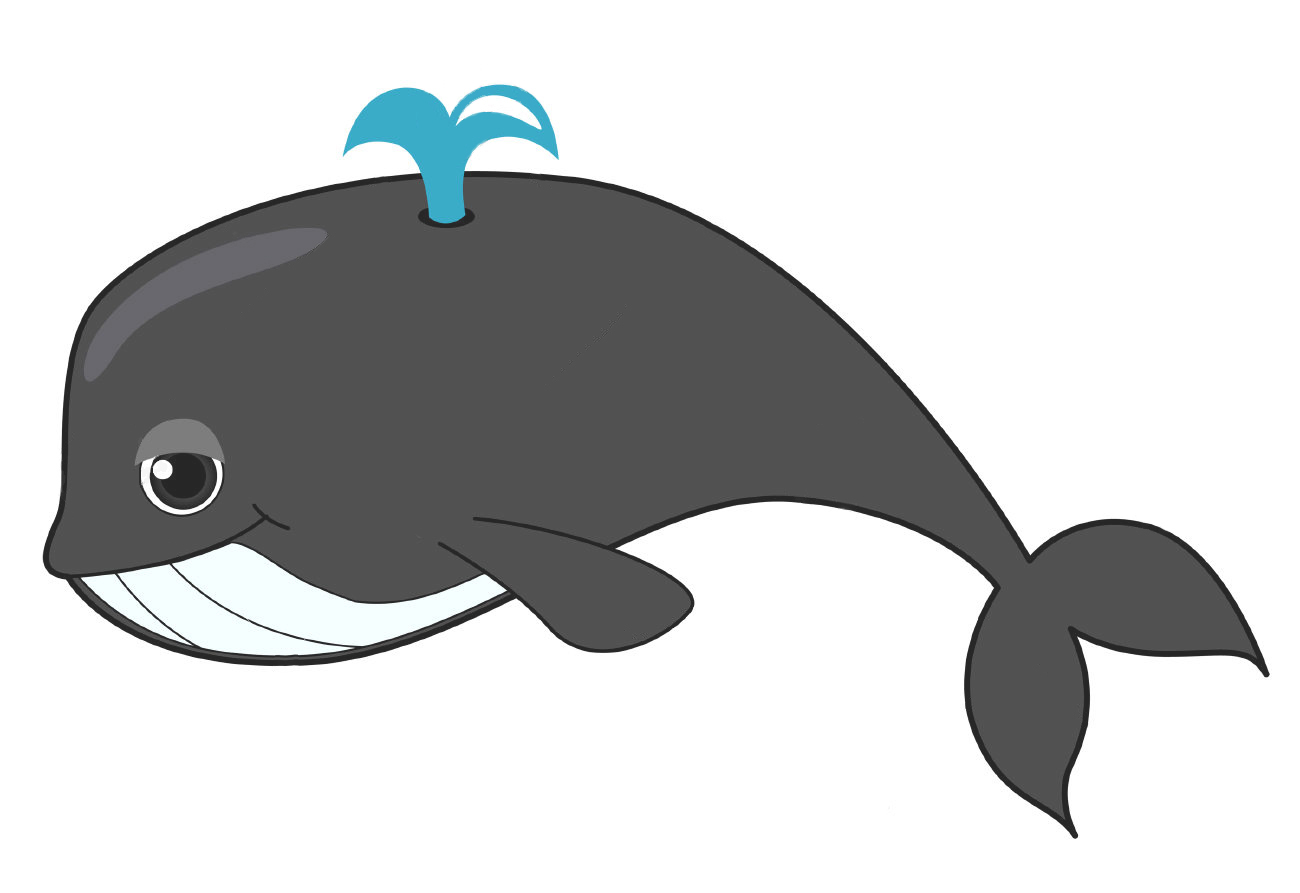
\includegraphics[scale=0.8]{graphics/clean_whale}
\end{center}




